\section{Kelvin-Helmholtz Instability} Kelvin-Helmholtz instability
is the mode of instability at the interface of two horizontal
parallel shear flows. The velocity profile is in general:
\begin{equation}\label{kh:pro}
\mathbf{U}(z) =
\begin{cases} U_1 \mathbf{i} &\text{if $z>0$,}
\\
U_2 \mathbf{i} &\text{if $z<0$.}
\end{cases}
\end{equation}
\begin{figure}[htpb]
  \centering
  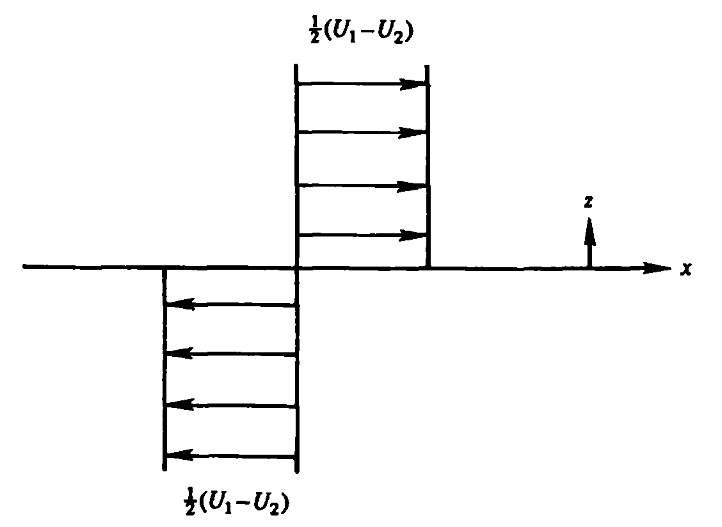
\includegraphics[width=0.9\textheight]{khpro.png}\\
  \caption{Velocity profile of a Kelvin-Helmholtz mode}\label{khpro}
\end{figure}

Kelvin-Helmholtz modes of instability is well found in the nature.
Figure \ref{khphoto} shows a billow cloud with the shape of
Kelvin-Helmholtz mode of waves.
\begin{figure}[htpb]
  \centering
  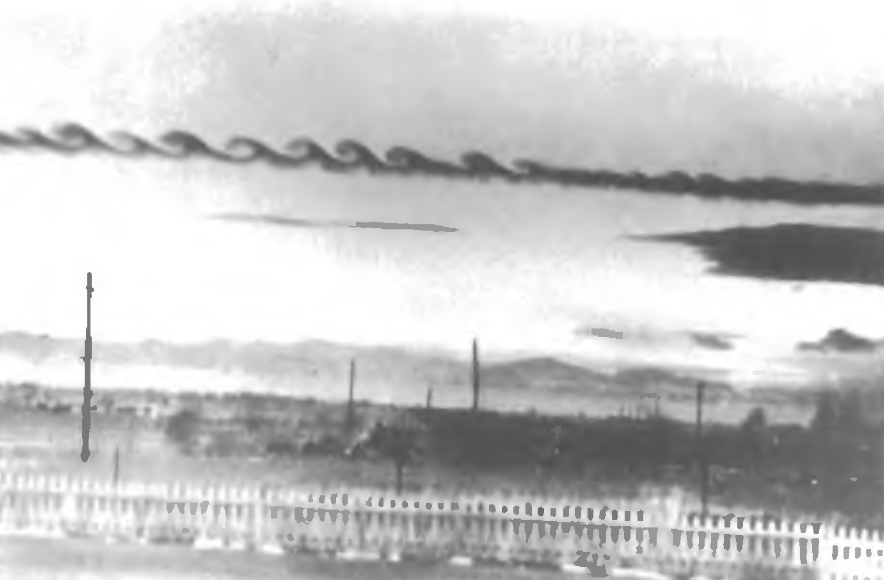
\includegraphics[width=0.9\textwidth]{khphoto.png}\\
  \caption{Billow cloud near Denver, Colorado (from \emph{Hydrodynamic Stability} by Drazin and Weid, \cite{Drazin})}\label{khphoto}
\end{figure}
